\documentclass{article}
\usepackage[utf8]{inputenc}
\usepackage{graphicx}
\usepackage[spanish]{babel}
\usepackage{amssymb,amsmath,geometry}
\usepackage[hidelinks]{hyperref}
\usepackage{etoolbox} %titulo
\makeatletter %titulo
\patchcmd{\@maketitle}{\vskip 2em}{\vspace*{-3cm}}{}{} %titulo
\makeatother %titulo
\usepackage{vmargin}
\setpapersize{A4}
\setmargins{2.5cm}       % margen izquierdo
{1.5cm}                        % margen superior
{16.5cm}                      % anchura del texto
{23.42cm}                    % altura del texto
{10pt}                           % altura de los encabezados
{1cm}                           % espacio entre el texto y los encabezados
{0pt}                             % altura del pie de página
{2cm}                           % espacio entre el texto y el pie de página
\title{Curvas y superfícies}
\author{Andoni Latorre Galarraga}
\date{}
\begin{document}
\setlength{\parindent}{0cm}
\newcommand{\norma}[1]{\left\|#1\right\|}
\maketitle

\section{Curvas}

\subsection{Curvas parametrizadas regulares}

%CPR

\textbf{Definición:}\\
Una \textit{curva parametrizada} (diferenciable) es una aplicación difrenciable $C^\infty$, $\alpha:(a,b)\subset\mathbb{R}\longrightarrow\mathbb{R}^n$ (donde $a$ y $b$ pueden ser $-\infty$ y $+\infty$ respectivamente). Decimos que $\alpha(t)=(x_1(t),\cdots,x_n(t))$ es $C^\infty$ si $x_i$ es $C^\infty$ $\forall i$.\\\\

%VELOCIDAD/TANGENTE

\textbf{Definición:}\\
Al vector $\alpha^\prime(t)=(x_1^\prime(t),\cdots,x_n^\prime(t))$ se le llama \textit{vector tangente (o velocidad)} de $\alpha$ en $t\in(a,b)$.\\\\

%EJEMPLOS

\textbf{Ejemplo1:}
\begin{center}
    \url{https://www.geogebra.org/3d/gyeab6be}\\
    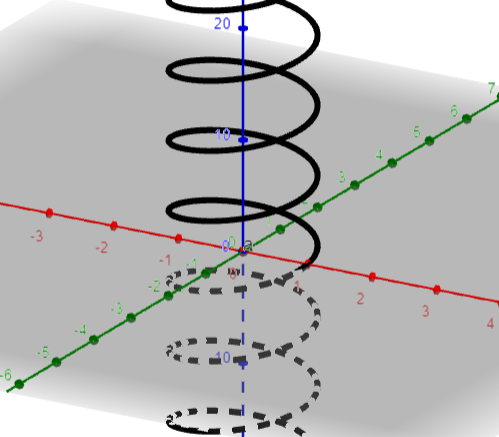
\includegraphics[scale=0.3]{figuras/ejemplos 1/sacacorchos.PNG}\\
    $\begin{array}{cccl}
    \alpha\::&\mathbb{R}&\longrightarrow&\mathbb{R}^3\\
        &t&\longmapsto&(\cos(t),\sin(t),t)
\end{array} \quad \alpha'(t)=(\sin(t),\cos(t),1$
\end{center}
\textbf{Ejemplo 2:}
\begin{center}
    \url{https://www.geogebra.org/calculator/vjehmjyh}\\
    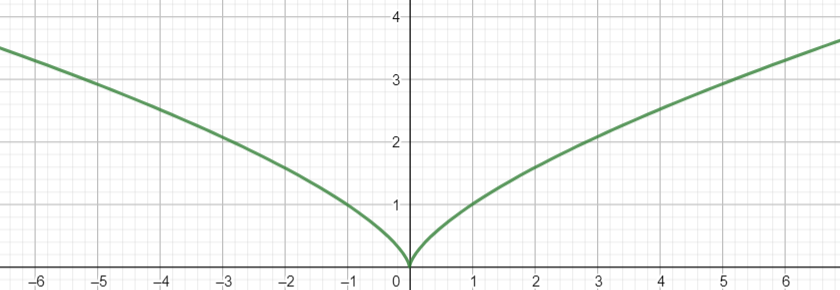
\includegraphics[scale=0.4]{figuras/ejemplos 1/ejemplo punto singular.PNG}\\
    $\begin{array}{cccl}
    \alpha\::&\mathbb{R}&\longrightarrow&\mathbb{R}^2\\
        &t&\longmapsto&(t^3,t^2)
\end{array} \quad \alpha'(t)=(3t^2,2t$\\
Punto singular en $t=0$ ya que $\alpha'(0)=(0,0)$
\end{center}
\textbf{Ejemplo 3:}
\begin{center}
    \url{https://www.geogebra.org/calculator/une2dbyd}\\
    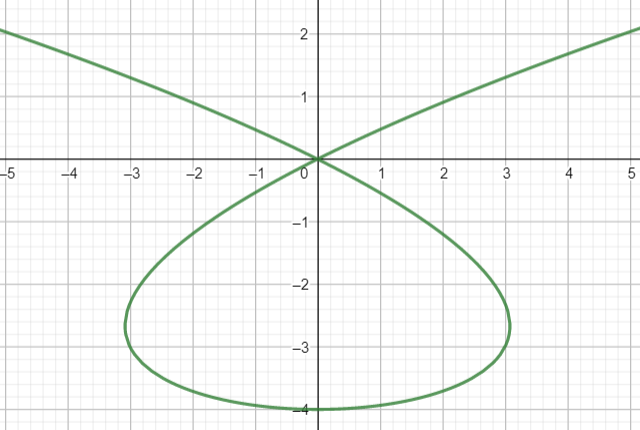
\includegraphics[scale=0.4]{figuras/ejemplos 1/ejemplo 3.PNG}\\
    $\begin{array}{cccl}
    \alpha\::&\mathbb{R}&\longrightarrow&\mathbb{R}^2\\
        &t&\longmapsto&(t^3-4t,t^2-4)
\end{array} \quad \alpha'(t)=3t^2-4,3t$\\
Como $\alpha(2)=\alpha(-2)=(0,0)$ no es inyectiva, pero $\alpha'(2)=(8,4)\ne\alpha'(-2)=(8,-4)$
\end{center}\newpage

\textbf{Ejemplo 4:}
\begin{center}
    \url{https://www.geogebra.org/calculator/hc2fvbne}\\
    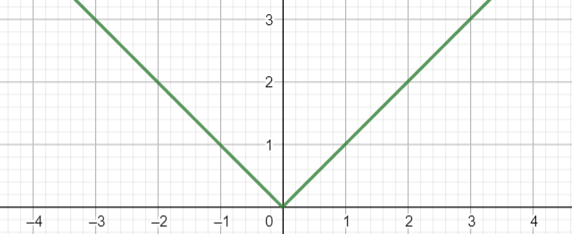
\includegraphics[scale=0.5]{figuras/ejemplos 1/ejemplo 4.PNG}\\
    $\begin{array}{cccl}
    \alpha\::&\mathbb{R}&\longrightarrow&\mathbb{R}^2\\
        &t&\longmapsto&(t,|t|)
\end{array} \quad \left\{\begin{array}{lll}
    \alpha(t)=(t,t) & \alpha'(t)=(1,1) & t>0 \\
    \alpha(t)=(t,-t) & \alpha'(t)=(1,-1) & t<0
\end{array}\right.$\\
No es de clase $\mathcal{C}^\infty$
\end{center}
\textbf{Ejemplo 5:}
\begin{center}
    \url{https://www.geogebra.org/calculator/tbb8nj9u}\\
    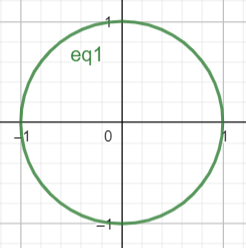
\includegraphics[scale=0.5]{figuras/ejemplos 1/ejemplo circulo.PNG}\\
    $\begin{array}{cccl}
    \alpha\::&\mathbb{R}&\longrightarrow&\mathbb{R}^2\\
        &t&\longmapsto&(\cos(t),\sin(t))
\end{array} \quad \alpha'(t)=(-\sin(t),\cos(t))$\\
    $\begin{array}{cccl}
    \beta\::&\mathbb{R}&\longrightarrow&\mathbb{R}^2\\
        &t&\longmapsto&(\cos(2t),\sin(2t))
\end{array} \quad \beta'(t)=2(-\sin(t),\cos(t))$
\end{center}

%RECTA TANGENTE

\textbf{Definición:}\\
Sea $\alpha\::\:(a,b)\longrightarrow\mathbb{R}^n$ una curva parametrizada $\in\mathcal{C}^\infty$(se asume) para cada $t\in(a,b)$ tal que $\alpha'(t)\ne0$, existe una recta bien definida, que pasa por t y tiene dirección $\alpha'(t)$, se llama \textit{recta tangente} a $\alpha$ en $t$ (respectivamente $\alpha(t)$).\\\\

%RECTA TANGENTE LIMITE SECANTES

\textbf{Proposición:}\\
Sea $\alpha\::\:(a,b)\longrightarrow\mathbb{R}^n$ una curva parametrizada, para cada $t_0 \in (a,b)$ la tecta tangente en $t_0$ es el límite de las rectas secantes que pasan por $\alpha(t)$ y $\alpha(t_0)$ cuando $t\to t_0$
\begin{center}
    \url{https://www.geogebra.org/calculator/hgbhfd2r}\\
    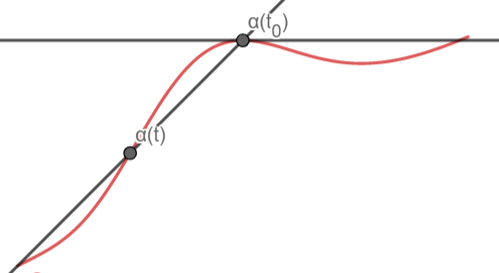
\includegraphics[scale=0.5]{figuras/limite secantes/limite secantes 1.PNG}
    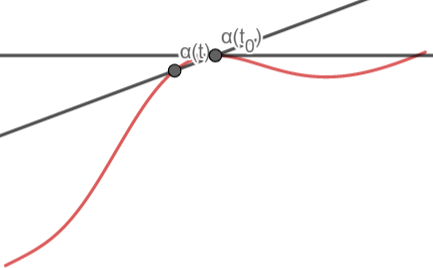
\includegraphics[scale=0.5]{figuras/limite secantes/limitew secantes 2.PNG}
\end{center}
\textit{Dem:}\\
$\alpha'(t_0)=\lim_{t\to t_0} \frac{\alpha(t)-\alpha(t_0)}{t-t_0}$.\\\\

%CURVA REGULAR

\textbf{Definición:}\\
Sea $\alpha\::\:(a,b)\longrightarrow\mathbb{R}^n$ una curva parametrizada. $\alpha$ se dice \textit{regular} si $\alpha'(t)\ne0 \: \forall t \in(a,b)$.\\\\

%REPARAMETRIZACIÓN

\textbf{Definición:}\\
Sean $\alpha\::\:(a,b)\longrightarrow\mathbb{R}^n$ $\beta\::\:(a,b)\longrightarrow\mathbb{R}^n$ curvas parametrizadas. $\beta$ es una \textit{reparamertrización} de $\alpha$ si existe $h\::\:(c,d)\longrightarrow(a,b)\in \mathcal{C}^\infty$ tal que $h'(s)\ne 0 \: \forall s\in (c,d)$ y $\beta=\alpha\circ h$.\\\\%%esquemita?


%NOTA VECTOR TANGETE NO GEOMETRICO

\textbf{Nota:}\\
El vector tangente no es geometrico en el sentido de que cambia con la reparametrización.\\\\

%TANGENTE REPARAMETRIZACION

\textbf{Lema:}\\
Sea $\beta$ reparametrización de $\alpha$, entonces $\beta'(u)=h'(u)\alpha'(h(u))\:\forall u\in(c,d)$.\\
\textit{Dem:}\\
Regla de la cadena.\\\\

%RECTA TANGENTE GEOMETRICA

\textbf{Proposición:}\\
En los puntos regulares de la curva la recta tangente es geométrica (no cambia con la reparametrización).\\
\textit{Dem:}\\
Vemos que el vector tangente de $\beta$ es proporcional al de $\alpha$ en cada punto (posiblemente con diferente proporcionalidad en cada punto) por el lema anterior.\\\\

%OBJETO GEOMETRICO

\textbf{Definición:}\\
Se dice que un objeto es \textit{geométrico} si es invariante respecto a reparametrizaciones o movimientos euclideos (translaciones y rotaciones).

%LONGITUD

\textbf{Definición:}\\
Sea $\alpha\::\:[a,b]\longrightarrow\mathbb{R}^n$ una curva parametrizada. Definimos \textit{longitud} de $\alpha$ en el intervalo $[a,b]$ como
$$
L_{[a,b]}(\alpha)=\int_a^b \norma{\alpha'(t)} dt
$$

%LONGITUD GEOMETRICO

\textbf{Proposición:}\\
La longitud es invariante respecto a movimientos euclídeos.\\
\textbf{Dem:}
Sea $\beta$ una parametrización de $\alpha$, entonces se verifica que $L(\beta)=L(\alpha)$.\\
$$
L(\beta)=\int_c^d |h's|\cdot \norma{\alpha'(h(s))} ds
$$
Si $h$ es creciente, $h'(s)>0 \: \forall s\in(c,d)$
$$
L(\beta)=\int_c^d h's\cdot \norma{\alpha'(h(s))} ds
$$
Tenemos que $h(a)=c$ y $h(b)=d$.
$$
=\int_a^b \norma{\alpha'(t)}dt=L(\alpha)
$$
Si $h$ es decreciente, $h'(s)<0 \: \forall s\in(c,d)$
$$
L(\beta)=\int_c^d -h's\cdot \norma{\alpha'(h(s))} ds
$$
Tenemos que $h(b)=c$ y $h(a)=d$.
$$
=-\int_b^a \norma{\alpha'(t)}dt=\int_a^b \norma{\alpha'(t)}dt=L(\alpha)
$$
Se tiene que la longitud es un objeto geometrico respecto a reparametrizaciones.\\
Sea $A$ una matriz ortogonal y $b\in\mathbb{R}^n$ veamos que $L(\alpha)=L(A\alpha+b)$. Si $\beta(t)=A\alpha(t)+b$, entonces $\beta'(t)=A\alpha'(t)$, por ser $A$ ortogonal.
$$
\norma{A\alpha'(t))}=\norma{\alpha'(t)} \quad \Rightarrow \quad L(\alpha)=L(\beta)
$$

%ACOTACION DISTANCIA

\textbf{Proposición:}\\
$\norma{\alpha(a)-\alpha(b)}\le L_{[a,b]}(\alpha)$.\\
\textit{Dem:}\\
Por la desigualdad de Schwarz.
$$
\norma{\int_a^b \alpha'(t) dt}\le \int_a^b\norma{\alpha'(t)} dt
$$
$$
\norma{\int_a^b \alpha'(t) dt}\le L_{[a,b]}
$$
Por el teorema fundamental del cálculo,
$$
\norma{\alpha(b)-\alpha(a)}\le L_{[a,b]}
$$
Además $\norma{\alpha(b)-\alpha(a)}= |-1|\cdot\norma{\alpha(a)-\alpha(b)}=\norma{\alpha(a)-\alpha(b)}$.\\

%LONGITUD DE ARCO

\textbf{Definición:}\\
Dada una curva parametrizada regular $\alpha\::\:[a,b]\longrightarrow\mathbb{R}^n$ para $c\in(a,b)$ se define la \textit{longitud de arco} (empezando en c) como la función
$$
s_\alpha(t)=\int_c^t\norma{\alpha'(u)}du \quad \forall t\in(a,b)
$$

%LOONGITUD DE ARCO = LONGITUD NORMAL

\textbf{Nota:}\\
$s_\alpha(t)=L_{[c,t]}(\alpha)$.\\\\

%EXISTE REPARAMETRIZACIÓN UNITARIA

\textbf{Teorema:}\\
Sea $\alpha\::\:[a,b]\longrightarrow\mathbb{R}^n$ un curva parametrizada regular, entonces existe una repametrización $\beta$ con velocidad unitaria, es decir, $\norma{\beta'(s)}=1\:\forall s$.\\
\textit{Dem:}\\
Por el teorema fundamental del cálculo,
$$
s_\alpha(t)=\int_c^t\norma{\alpha'(u)}du \quad \forall t\in(a,b)\quad\Rightarrow\quad\frac{ds}{dt}(t)=\norma{\alpha'(t)}>0
$$
Como $\frac{ds}{dt}\ne0$ por el teorema de la función inversa existe $t(s)\::s(t)\to t$ y
$$
\frac{dt}{ds}(s)=\frac{1}{\frac{ds}{dt}(t)}
$$
Sea $\beta(s)=\alpha(t(s))$, se tiene
$$
\beta'(s)=\alpha'(t(s))t'(s)\quad \norma{\beta'(s)}=\norma{\alpha'(t(s))}\frac{1}{s'(t(s))}=\norma{\alpha'(t(s))}\frac{1}{\norma{\alpha'(t(s))}}=1
$$

%EJEMPLO PARAMETRIZACIÓN UNITARIA

\textbf{Ejemplo:}\\
$\alpha\::\:\mathbb{R}\longrightarrow\mathbb{R}^3$ donde $\alpha(t)=(a\cos(t),a\sin(t),bt)$.
$$
\alpha'(t)=(-a\sin(t),a\cos(t),b) \quad \norma{\alpha'(t)}=\sqrt{a^2\sin^2(t)+a`2\cos^2(t)+b^2}=\sqrt{a^2+b^2}\ne0
$$
Por lo que $\alpha$ es regular.
$$
s(t)=\int_0^t\norma{\alpha'(u)}du=\sqrt{a^2+b^2}t
$$
Se tiene que $\bar{\alpha}(t)=\left(a\cos\left(\frac{s}{\sqrt{a^2+b^2}}\right),a\sin\left(\frac{s}{\sqrt{a^2+b^2}}\right),b\frac{s}{\sqrt{a^2+b^2}}\right)$.\newpage


\subsection{Teoría local de curvas planas}

%J

\textbf{Nota:}\\
$\mathcal{J}(x,y)=(-y,x)$.\\

%DIEDRO DE FRENET/CURVATURA

\textbf{Definición:}\\
Sea $\alpha\::(a,b)\longrightarrow\mathbb{R}^2$ una curva parametrizada regular que está parametrizada por longitud de arco. El \textit{diedro de Frenet} es una base ortonormal positivamente orientada $(\mathbb{T}(s),\mathbb{N}(s)$ tal que
$$
\mathbb{T}(s)=\alpha'(s)
$$
$$
\left\{\begin{array}{l}
    \mathbb{T}(s)\mathbb{N}(s)=0\\
    \norma{\mathbb{N}(s)}\\
    \det(\mathbb{T}(s),\mathbb{N}(s))>0
\end{array}\right.\quad
\mathbb{N}(s)=\mathcal{J}(\mathbb{T}(s))
$$
\begin{center}
    \url{https://www.geogebra.org/calculator/syjbfepp}\\
    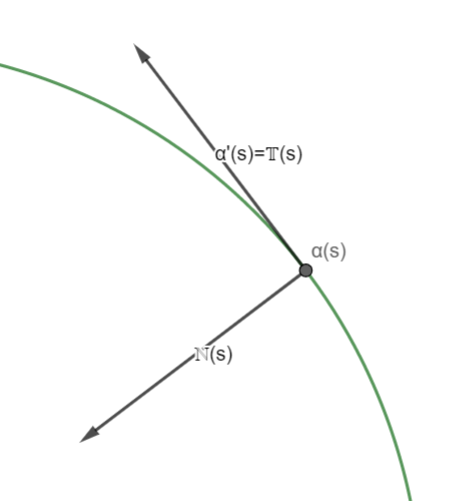
\includegraphics[scale=0.5]{figuras/Diedro de frenet.PNG}
\end{center}
Veamos que ocurre si intentamos escribir $\mathbb{T}'(s)$ y $\mathbb{N}'(s)$ en la base $\mathbb{T}(s),\mathbb{N}(s)$. Observamos que
$$
\norma{\mathbb{T}(s)}=1\quad\Rightarrow\quad\mathbb{T}(s)\mathbb{T}(s)\quad\Rightarrow\quad\underbrace{\mathbb{T}'(s)\mathbb{T}(s)=0}_{\text{componente de $\mathbb{T}'(s)$ en $\mathbb{T}(s)$}}
$$
$$
\norma{\mathbb{N}(s)}=1\quad\Rightarrow\quad\mathbb{N}(s)\mathbb{N}(s)\quad\Rightarrow\quad\underbrace{\mathbb{N}'(s)\mathbb{N}(s)=0}_{\text{componente de $\mathbb{N}'(s)$ en $\mathbb{N}(s)$}}
$$
Por lo tanto,
$$
\left\{\begin{array}{l}
    \mathbb{T}'(s)=0\cdot\mathbb{T}+b(s)\cdot\mathbb{N}\\
    \mathbb{N}'(s)=c(s)\cdot\mathbb{T}+0\cdot\mathbb{N}
\end{array}\right.
$$
Por otra parte,
$$
\mathbb{T}(s)\cdot\mathbb{N}(s)=0\quad\Rightarrow\quad\mathbb{T}'(s)\cdot\mathbb{N}(s)+\mathbb{N}'(s)\cdot\mathbb{T}(s)=0\quad\Rightarrow\quad\mathbb{T}'(s)\cdot\mathbb{N}(s)=-\mathbb{T}(s)\cdot\mathbb{N}'(s)
$$
Entonces tiene sentido definir
$$
c(s)=-k_2(s)=-b(s)
$$
Llamamos \textit{curvatura con signo} a $k_2(s)$. También tenemos las \textit{fórmulas de Frenet}
$$
\left\{\begin{array}{l}
    \mathbb{T}'(s)=k_2(s)\cdot\mathbb{N}(s)\\
    \mathbb{N}'(s)=-k_2(s)\cdot\mathbb{T}(s)
\end{array}\right.
$$
Además,
$$
\mathbb{T}(s)=\alpha'(s),
\mathbb{N}(s)=\mathcal{J}\alpha'(s)
$$
$$
\mathbb{T}'(s)=\alpha''(s)=k_2(s)\mathcal{J}\alpha'(s)
$$
$$
\alpha''(s)\mathcal{J}\alpha'(s)=k_2(s)\mathcal{J}\alpha'(s)\mathcal{J}\alpha'(s)=k_2(s)
$$
$$
k_2(s)=\alpha''(s)\mathcal{J}\alpha'(s)
$$\newpage

\textbf{Nota:}\\
$|k_2(s)|=\norma{\alpha'(s)}$ y $\alpha''(s)$ apunta en la dirección en la que se curva la curva. Cuando la curtvatura es positiva se curva con $\mathbb{N}(s)$ y cuando la curvatura es negativa se curva contra $\mathbb{N}(s)$.\\\\

%EJEMPLOS CURVATURA

\textbf{Ejemplo 1:}\\
\textbf{Ejemplo 2:}\\
\\\\

%CUALQUIER PARAMETRIZACIÓN

\textbf{Definición:}\\
Sea $\alpha\::(a,b)\longrightarrow\mathbb{R}^2$ una curva parametrizada (no necesariamente parametrizada por longitud de arco). Si $s(t)$ es la longitud de arco de $\alpha$
\end{document}